\documentclass[12pt,a4paper]{ctexart}

% === 页面设置 ===
\usepackage{geometry}
\geometry{left=1.8cm, right=1.8cm, top=2cm, bottom=1.5cm}

% === 包 ===
\usepackage{multirow}
\usepackage{makecell}
\usepackage{graphicx}
\usepackage{array}
\usepackage{calc}
\usepackage{longtable}

% === 表格列宽（7列，总宽=\textwidth） ===
% 列0: 标签  列1: 值  列2: 标签  列3: 值  列4: 标签  列5: 值  列6: 照片
\newlength{\colzero}\setlength{\colzero}{2.2cm}
\newlength{\colone}\setlength{\colone}{2.5cm}
\newlength{\coltwo}\setlength{\coltwo}{1.0cm}
\newlength{\colthree}\setlength{\colthree}{2.2cm}
\newlength{\colfour}\setlength{\colfour}{1.4cm}
\newlength{\colfive}\setlength{\colfive}{2.2cm}
\newlength{\colsix}\setlength{\colsix}{2.2cm}

% 合并列1-6的宽度（用于底部长文本区）
\newlength{\colmerge}
\setlength{\colmerge}{\dimexpr\colone+\coltwo+\colthree+\colfour+\colfive+\colsix+10\tabcolsep\relax}

% 合并列2-4的宽度（用于"专业排名/专业人数"标签）
\newlength{\colmidmerge}
\setlength{\colmidmerge}{\dimexpr\coltwo+\colthree+\colfour+4\tabcolsep\relax}

% === 辅助命令 ===
\newcommand{\lbl}[1]{\textbf{#1}}       % 标签格（宋体加粗）
\newcommand{\val}[1]{#1}                % 内容格（仿宋）

\begin{document}

\setlength{\extrarowheight}{6pt}
\setlength{\LTpre}{0pt}
\setlength{\LTpost}{0pt}

\begin{longtable}{|p{\colzero}|p{\colone}|p{\coltwo}|p{\colthree}|p{\colfour}|p{\colfive}|p{\colsix}|}
\hline
% === 第0行：标题 ===
\multicolumn{7}{|c|}{\textbf{\zihao{3} 中南大学自动化学院2026级新生带班学长学姐申请表}} \\
\hline
% === 第1行：填表日期 ===
\multicolumn{7}{|c|}{\zihao{-4} 填表日期：\hspace{1.5cm}年\hspace{1cm}月\hspace{1cm}日} \\
\hline
% === 第2行：姓名、性别、年龄 + 照片（4行合并）===
\centering\lbl{姓\ \ 名} & \centering\val{陈威宇} &
\centering\lbl{性\ \ 别} & \centering\val{男} &
\centering\lbl{年\ \ 龄} & \centering\val{21} &
\multirow{4}{2cm}{\centering\raisebox{-0.3cm}{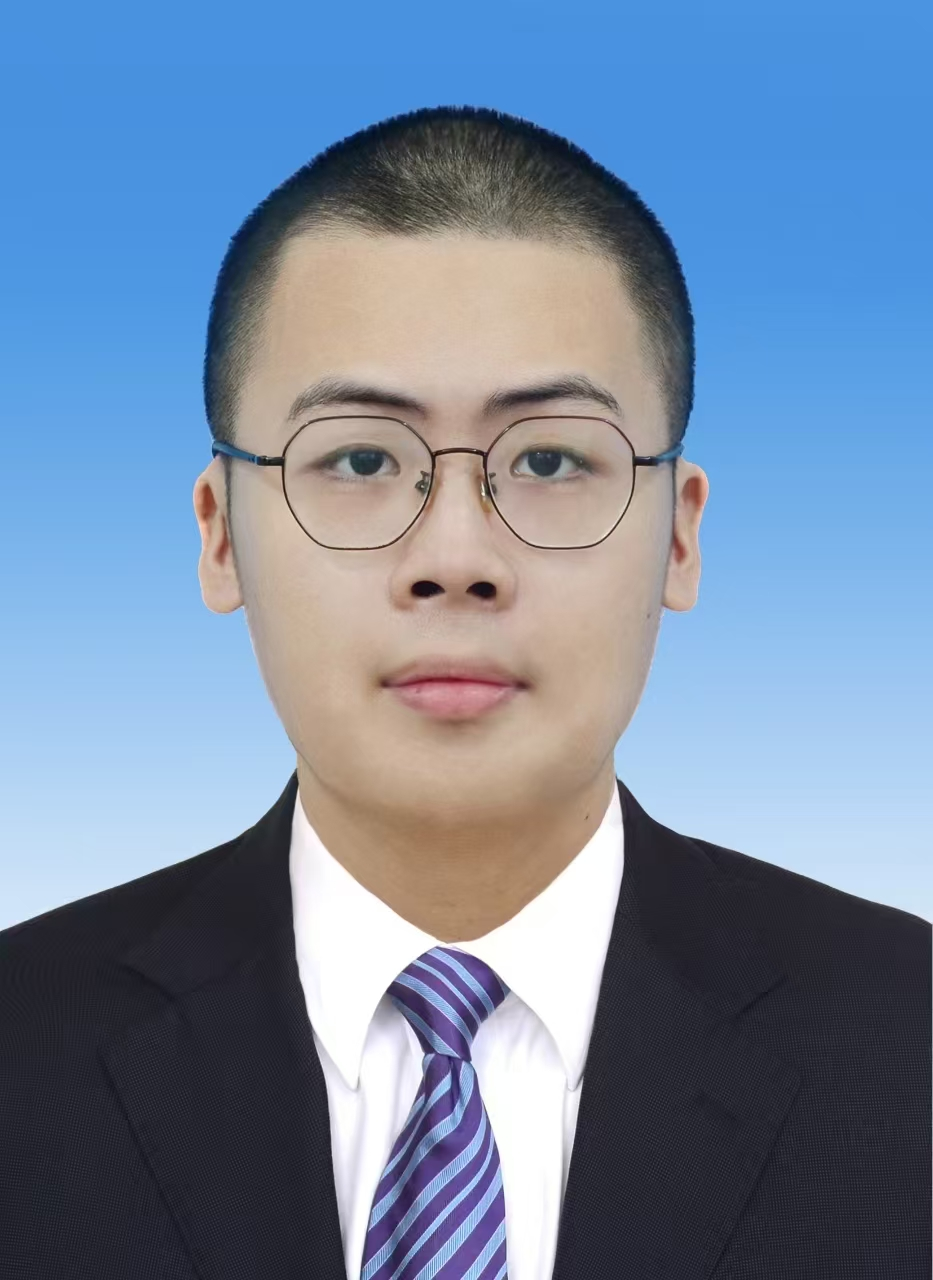
\includegraphics[width=1.8cm]{微信图片_20251018145143_216_33.jpg}}} \\
\cline{1-6}
% === 第3行：专业、班级、政治面貌 ===
\centering\lbl{专\ \ 业} & \centering\val{自动化卓越人才培养} &
\centering\lbl{班\ \ 级} & \centering\val{自动化T2301} &
\centering\lbl{政治面貌} & \centering\val{中共预备党员} & \\
\cline{1-6}
% === 第4行：联系电话、QQ、微信 ===
\centering\lbl{联系电话} & \centering\val{13607585678} &
\centering\lbl{QQ} & \centering\val{2993139719} &
\centering\lbl{微\ \ 信} & \centering\val{sutao2208} & \\
\cline{1-6}
% === 第5行：籍贯、专业排名 ===
\centering\lbl{籍\ \ 贯} & \centering\val{福建漳州} &
\multicolumn{3}{p{\colmidmerge}|}{\centering\lbl{专业排名/专业人数}} &
\centering\val{4/29} & \\
\hline
% === 第6行：个人爱好 ===
\centering\lbl{个人爱好} &
\multicolumn{6}{p{\colmerge}|}{\val{跑步、旅游、探索美食、研究数学题}} \\
\hline
% ====== 第7行：学生工作经历（拆成5个子行，longtable可在任意子行间断页）======
\centering\lbl{学生工作经历} &
\multicolumn{6}{p{\colmerge}|}{{\zihao{5}\lbl{（时间，组织或活动名称，担任职务或角色，主要工作及实际成效）}}} \\
\cline{2-7}
 &
\multicolumn{6}{p{\colmerge}|}{{\zihao{5}2023.9--2024.6\ \ 共青团中南大学委员会社团部（现社团管理中心）新媒体运营中心（现宣传部）干事。负责百团大战现场组织协调，社团活动宣传推送制作，阅读量2000+。}} \\
\cline{2-7}
 &
\multicolumn{6}{p{\colmerge}|}{{\zihao{5}2024.2--至今\ \ 担任中南大学自动化学院自动化卓越人才培养T2301班宣传委员、文宣委员。负责班级活动团日活动有关记录和宣传。自动化学院2023级卓越班召开师生座谈会文章发布在中南大学自动化学院官网，累计浏览近千次。}} \\
\cline{2-7}
 &
\multicolumn{6}{p{\colmerge}|}{{\zihao{5}2024.9--至今\ \ 在中南大学自动化学院规学堂学业辅导站任职。其中2024.9--2025.8任宣学站干事，负责学院辅学活动推文制作工作和学风建设活动协助工作；2025.9--至今任督学站站长，负责学院辅学义工招新和日常活动的组织管理。主持学院第二十一期发展对象（预备党员）鸿雁领航党员帮扶活动，改进活动组织方式，提高了党员的参与率与成效。}} \\
\cline{2-7}
 &
\multicolumn{6}{p{\colmerge}|}{{\zihao{5}2023.9--至今\ \ 在中南自习社担任社团干事，教研部部员。负责社团高等数学期中模拟题命制与每日一题命制。有关题目连续两年（2024、2025）被中南大学材料科学与工程学院学习部用作期中测试题。2025年我将高等数学试题扫描成\LaTeX 实现期末真题的标准化与规范化，并无偿分享。}} \\
\hline
% ====== 第8行：申请动机及岗位认识（拆成4个子行）======
\centering\lbl{申请动机及岗位认识} &
\multicolumn{6}{p{\colmerge}|}{{\zihao{5}\lbl{（你为什么想担任带班学长学姐？你觉得这个岗位需要做哪些事情？）}}} \\
\cline{2-7}
 &
\multicolumn{6}{p{\colmerge}|}{{\zihao{5}在我初入大学的时候，有许多优秀的学长学姐在帮助我适应大学生活。比如工力2201班的苗继凯学长，他当班助的认真负责，作为学长的优秀，让我入学时就办理好了各项手续，以更加昂扬的精神姿态面对学习。还有土木院分配的一对一学长陈宇航学长（转专业到电科）也让我更加确信通过我的努力是可以在竞争激烈的土木院实现转专业。随着期末的接近，卓越班选拔通知下发。我有幸认识了自动化学院自动化专业的柳博文学长，自动化卓越人才培养的李信开、郭逍遥、汤淼学长。}} \\
\cline{2-7}
 &
\multicolumn{6}{p{\colmerge}|}{{\zihao{5}他们为我备考卓越班选拔考核，进入自动化学院，进入卓越班后适应班内竞争环境，在新的起点上努力学习争取更高成绩提供了许多宝贵经验和建议；他们也身体力行，是我的榜样。柳博文学长分享了许多宝贵的学习资料；李信开学长成绩不断进步，加入规学站担任帮学站站长，大三学年综测第一最后本校本博计划入选；后续面临保研准备，卓越人才培养的王易衡学长也为我了解保研情况与去向提供了许多帮助。还有鲍嘉祺学长、郭伊扬学长也都持续参与志愿服务活动的同时，加权综测成绩不断进步。在他们的帮助和精神鼓舞下，我进班后加权不断进步，从进班的$17\rightarrow8\rightarrow7\rightarrow5\rightarrow4$，不断进步，获得企业奖学金，优秀学生与优秀学生干部，获得省级竞赛奖项。}} \\
\cline{2-7}
 &
\multicolumn{6}{p{\colmerge}|}{{\zihao{5}在大学这四年里，我在学习成绩的取得上、竞赛科研的参与上、课外活动学生工作等的参加上积累了许多宝贵的经验。有些可能是成功的，比如加权成绩上；有些可能是错题集，比如竞赛参加上，这也是大学的一大遗憾。除此之外在平时我也经常在有空闲的时间，无偿的，尽己所能帮助许多同学。有许多同学也取得了很不错的成绩。我希望把这个精神继续传承下去，帮助更多的新生学弟学妹尽快适应大学生活，少走弯路，取得更好的发展。}\vspace*{1.5cm}} \\
\hline
% === 第9行：带班工作初步设想 ===
\centering\lbl{带班工作初步设想} &
\multicolumn{6}{p{\colmerge}|}{{\zihao{5}\lbl{（你认为新生入学后最容易遇到哪些问题？如被选为带班学长学姐，你准备从哪些方面帮助新生完成学习、生活和人际适应，做好班级建设？）}}\vspace*{3.0cm}} \\
\hline
% === 第10行：自我评价 ===
\centering\lbl{自我评价} &
\multicolumn{6}{p{\colmerge}|}{\vspace*{2.8cm}} \\
\hline
% === 第11行：其他需要说明的问题 ===
\centering\lbl{其他需要说明的问题} &
\multicolumn{6}{p{\colmerge}|}{\vspace*{2.8cm}} \\
\hline
\end{longtable}

\end{document}
